\documentclass{article}
\usepackage{graphicx}
\graphicspath{./diagrams}
\usepackage{mathtools}
\usepackage{amsfonts}
\usepackage{amssymb}
\usepackage{amsmath}
\usepackage{amsthm}
\usepackage{physics}
\usepackage{pgfplots}
\pgfplotsset{compat=1.18}

\newtheorem{definition}{Definition}[section]

\title{An Introduction to Complex Numbers}
\author{Joshua John Lee Shi Kai}

\begin{document}
\maketitle
\tableofcontents

\newpage
\section{Introduction}
Complex Analysis is quite similar to real analysis, except it works with complex numbers of the form
$x + iy$, where $x, y \in \mathbb{R}, i^2 = -1$. We represent real numbers on a line, we represent complex
numbers as elements on a plane.

\noindent \\ For example:
\begin{center}
	\begin{tikzpicture}
		\begin{axis}[xmin=0,xmax=3,ymin=0,ymax=3,xlabel = $x$, ylabel = $i$, axis lines = middle]
			\fill (2,1) circle[radius = 2pt] node[above right]{$(2,1)$};
		\end{axis}

	\end{tikzpicture}

\end{center}

\noindent A lot of complex analysis is really similar to real analysis, we can do the usual $+, -, \times, /$,
exponentials, trignometric functions, differentiation, integration. Many of the rules for real analysis work for
complex analysis. $\lim$, series and so on...

\subsection{Some Differences}
\subsubsection{Euler: $e^{ix} = cosx + isinx$}
Trigonometric functions and exponential functions turn out to be almost the same.
Using this we can write all trignometric functions in terms of exponential functions for example,
$cosx = \frac{e^{ix} + e^{-ix}}{2}$. This saves a lot of labour because all the complicated identities
for trigonometric functions are just special cases of identities of exponential functions. So there's a lot
less to remember.
\subsubsection{Differentiability}
For the reals, some functions we can differentiate it once and twice, but not three times. But for a
complex function $\mathbb{C} \rightarrow \mathbb{C}$, once it is differentiable once, it is automatically
differentiable any number of times.
\subsubsection{Integration}
Suppose we want to integrate
\begin{displaymath}
	\int_{0}^{1}f(x)dx
\end{displaymath}
Suppose we want to integrate for real numbers, and there's only one way to go from 0 to 1.
\begin{center}
	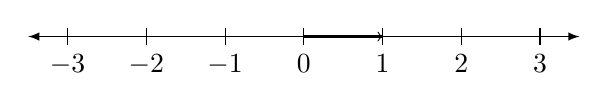
\begin{tikzpicture}
		\draw[latex-latex] (-3.5,0) -- (3.5,0) ; %edit here for the axis
		\foreach \x in  {-3,-2,-1,0,1,2,3} % edit here for the vertical lines
		\draw[shift={(\x,0)},color=black] (0pt,3pt) -- (0pt,-3pt);
		\foreach \x in {-3,-2,-1,0,1,2,3} % edit here for the numbers
		\draw[shift={(\x,0)},color=black] (0pt,0pt) -- (0pt,-3pt) node[below]
		{$\x$};
		\draw[->] (0,0) -- (1.0,0);
		\draw[very thick] (0,0) -- (1,0);
	\end{tikzpicture}
\end{center}
So its quite clear what this integral is meant.

\noindent \\ But if we are integrating in the complex plane,
\begin{center}
	\begin{tikzpicture}
		\begin{axis}[xmin=-1,xmax=3,ymin=-1,ymax=3,xlabel = $x$, ylabel = $i$, axis lines = middle]
			\fill (1,0) circle[radius = 2pt] node[above right]{$(1,0)$};
			\fill (0,1) circle[radius = 2pt] node[above right]{$(0,1)$};
			\addplot [
				domain=0:1,
				samples=150,
				color=blue,
			]
			{2*x - 2*x^2};
			\addplot [
				domain=0:1,
				samples=150,
				color=red,
			]
			{4*x - 4*x^2};
			\addplot [
				domain=0:1,
				samples=150,
				color=purple,
			]
			{-3*x + 3*x^2};

		\end{axis}
	\end{tikzpicture}
\end{center}
There are many ways to go from 0 to 1. So the integral from 0 to 1 seems to depend on which path you take.
Turns out that it almost doesn't. We have Cauch's theorem, that integrals are almost independent of the path
we take from 0 to 1. This turns out to extremely useful. For example in real analysis, there are some equations integrals and sums that we don't learn how to evaluate in ordinary
introductory calculus classes. But you can work out these using complex integration.
\begin{gather*}
	\int_{0}^{\infty}\frac{sinx}{x}dx = \frac{\pi}{2} \\
	\displaystyle\sum_{i=1}^{\infty} \frac{1}{1^2} + \frac{1}{2^2} + \frac{1}{3^2} + \cdots = \frac{\pi^2}{6}
\end{gather*}
\subsection{Analytic Continuation}
Suppose I give you a function from 0 to 1, and ask you to evaluate it at $x = -1$, that would be a
completely stupid question. There's no way to evaluate it at $-1$. There is no real information.
However for complex functions, if I give you a function from 0 to 1, and it is differentiable, it is
automatically determined in any connected region.

\noindent The function on $(a,b)$ is determined uniquely on larger open connected set if it complex differentiable.

\noindent There is a very famous function of this. The Riemann Zeta Function
\begin{displaymath}
	\zeta(s) = \frac{1}{1^s}	+ \frac{1}{2^s}	+ \frac{1}{3^s}	+ \cdots
\end{displaymath}
This is probably the single most notorious function in mathematics, the Riemann hypothesis, which
states that all zeros of $\zeta (s)$ are real or have real part of $\frac{1}{2}$

\begin{center}
	\begin{tikzpicture}
		\begin{axis}[
				legend pos=outer north east,
				title=Riemann Hypothesis,
				xmin=-1, xmax=3,
				ymin=-1, ymax=3,
				axis lines=middle,
				xlabel = $x$,
				ylabel = $i$,
				variable = x,
				trig format plots = rad,
			]

			\draw[purple, thick] (0.5, 3) -- (0.5, -1) node[left, pos=0.6] {$x=\frac{1}{2}$};
			\draw[blue, thick] (1, 3) -- (1, -1) node[right, pos=0.5] {$x=1$};
		\end{axis}
	\end{tikzpicture}
\end{center}
Well the Riemann Hypothesis makes no sense at all because if we try to evaluate it it only converges if
$\Re(s) > 1$
\begin{equation}
	1 + \frac{1}{2} + \frac{1}{3} + \cdots = \infty
\end{equation}
And the function only converges on the right side of $x = 1$. Well it turns out the Riemann Zeta
function can be analytically continued. In other words, there's only one differentiable complex function
that extends the Riemann Zeta function to the whole complex plane, except well, 1 because it would not
converge. Why should people care about the Riemann Zeta function? Well it seems to control prime numbers,
if we draw prime numbers on a real line,
\begin{center}
	\begin{tikzpicture}
		\draw[latex-latex] (0,0) -- (8,0) ; %edit here for the axis
		\foreach \x in  {2,3,5,7} % edit here for the vertical lines
		\draw[shift={(\x,0)},color=black] (0pt,3pt) -- (0pt,-3pt);
		\foreach \x in {2,3,5,7} % edit here for the numbers
		\draw[shift={(\x,0)},color=black] (0pt,0pt) -- (0pt,-3pt) node[below]
		{$\x$};
	\end{tikzpicture}
\end{center}
You can see that they are more dense in some regions, and in some regions
they are less dense. Something like a sort of compression wave. Riemann
discovered that this waves in the primes happen at very precise frequencies,
and the frequencies turn out to be the imaginary parts of the zeroes of the
zeta function. The amplitude of each wave turn out to be the real part. So
the Riemann Hypothesis seems to suggest that primes have a lot of waves going
through them. And all these waves in some sense have the same loudness, or volume.

\subsection{Complex Dynamics}
This is related to a planar set called the Mandel Brot set. We can ask what is the Mandel Brot set?

\noindent You take a complex number, you keep on applying the transformation, while c is fixed
\begin{center}
	\begin{tabular}{lll}
		$z$   & $\rightarrow z^{2} + c$  &                      \\
		$0$   & $\rightarrow 0^{2} + c $ & $\rightarrow \cdots$ \\
		$z_0$ & $\rightarrow z_1$        & $\rightarrow z_2$    \\
		      & $= z_0^2 + c$            & = $z_1^2 + c$        \\
	\end{tabular}
\end{center}
And you can ask whether this sequence is \textbf{bounded}. And this obviously depends on c.
So if this sequence is bounded, it is the same as saying c is in the Mandel Brot set. The thing is
that the Mandel Brot set is incredibly intricate.
\begin{center}
	\includegraphics[width=\textwidth]{/diagrams/mandelbrot}
\end{center}

\noindent \\ Well that's the end of the summary.

\section{Complex Arithmetic}
Well if you were a computer, a complex number is nothing more than an ordered pair of numbers $(x,y)$. But
if you were human you would write it as $x + iy$. But as a human, writing it as an ordered pair
is good too because you could understand it as a plane. So you could represent each complex number
as a point in a plane.
\begin{definition}[Addition]
	\begin{displaymath}
		(a + ib) + (c+id) = a+c+ib+id
	\end{displaymath}
\end{definition}
\begin{definition}[Multiplication]
	\begin{align*}
		(a,b)  \cdot (c,d)  & = (ac-bd, ad+bc)             \\
		(a + ib) (c + id)   & = ac + i^{2}bd + ibc + iad   \\
		\text{Since } i^{2} & = -1,                        \\
		                    & \Rightarrow ac-bd + i(bc+ad)
	\end{align*}
\end{definition}
\noindent That's why we remember complex numbers as $x+iy$ form, because
it makes multiplication trivial to remember.
\subsection{The usual stuff}
Does it satisfy the usual rules:
\begin{equation*}
	a(b+c) = ab+ac
	(ab)c = a(bc)
	\cdots
\end{equation*}
Well we could
\begin{enumerate}
	\item Do a long check which we won't do because its long and tedious
	\item Go to an abstract algebra course, and show that the definition of the complex numbers gives a ring
	      with all the usual stuff
\end{enumerate}
\subsection{Division}
Does $a+ib$ has an \textit{inverse} if it is $\neq 0$.

\subsubsection{Complex Conjugation}
Denoted by:
\begin{gather*}
	x + iy \rightarrow x - iy = \overline{x+iy}
\end{gather*}
The reason this turns up a lot is we said $i^{2} = -1$ but $-1$
actually has 2 squareroots because $(-i)^{2} = -1$. So when we talk about
a squareroot of $-1$ we don't really know which squareroot they
are talking about and turns out, they are completely equivalent. Anything
you can say about 1 squareroot you can say about the other squareroot.
So you can sort of flip them around without changing anything. Complex
conjugation actually \textit{preserves} all properties of the complex
numbers. For example:
\begin{gather*}
	\overline{z_{1}z_{2}} = \overline{z_1} \cdot \overline{z_2} \\
	\overline{z_{1}+z_{2}} = \overline{z_1} + \overline{z_2}
\end{gather*}
In fact, complex conjugation $z \rightarrow \overline{z}$ is an \textit{AUTOMORPHISM}
of the complex numbers, $\mathbb{C}$. If you've done a Galois Theory course, another way
of saying is this is the Galois group of the $\mathbb{C}/\mathbb{R}$ is
$\{1,\text{Complex Conjugation}\}$.

\noindent \\ So using complex conjugation, we can find the inverse of any
complex number as follows
\begin{align*}
	z              & = x+iy                                           \\
	z \overline{z} & = (x+iy)(x-iy)                                   \\
	               & = x^{2}+y^{2}                                    \\
	\frac{1 }{z }  & = \frac{\overline{z}}{z\overline{z}}             \\
	\frac{1}{x+iy} & = \frac{x-iy}{(x+iy)(x-iy)}                      \\
	               & = \frac{x-iy}{x^{2}+y^{2}}                       \\
	               & = \frac{x}{x^{2}+y^{2}} - i\frac{y}{x^{2}+y^{2}}
\end{align*}
What you should remember is to multiply the denominator by its complex conjugate. Division by complex
numbers is also reasonably easy.

\subsubsection{Absolute Value}
The absolute distance of $x$ from 0 is $x$ if $x>0$ and $-x$ if $(x<0)$. Similarly, for any complex
number $z$,
\begin{align*}
	z   & = x+iy                 \\
	|z| & = \sqrt{x^{2}+y^{2}}   \\
	    & = \sqrt{z\overline{z}}
\end{align*}
From this, then the following also follows,
\begin{gather*}
	|z_{1}z_{2}| = |z_{1}||z_{2}|
\end{gather*}
All the rules of absolute value also applies,
\begin{gather*}
	|z_{1}-z_{2}| \leq |z_{1}| + |z_{2}|
\end{gather*}
\subsubsection{Application for Complex Arithmetic}
Which integers are sums of 2 squares? Well we know that they are
closed under multiplication. Meaning that if two integers are the sum of two squares then so is
their product.
\begin{proof}
	Let's say we have two integers that are the some of two squares, then
	\begin{displaymath}
		(a^2+b^2)(c^2+d^2) = (ac-bd)^2 + (ad+bc)^2
	\end{displaymath}
	Well where on earth did this come from? It comes from complex numbers!
	We notice that
	\begin{align*}
		a^2+b^2            & = |a+ib|^2              \\
		c^2+d^2            & = |c+id|^2              \\
		(a^2+b^2)(c^2+d^2) & = |(a+ib)(c+id)|^2      \\
		                   & = |ac-bd + i(ad+bc)|^2  \\
		                   & = (ac-bd)^2 + (ad+bc)^2
	\end{align*}
\end{proof}
\noindent The proof with reals doesn't really explain why it exists, it is explained with
complex numbers.
\begin{proof}
	Let's give an example of this
	\begin{align*}
		5           & = 1^2 + 2^2     \\
		13          & = 2^2 + 3^2     \\
		5 \times 13 & = 65            \\
		            & = 8^{2} + 1^{2} \\
		            & = 4^{2} + 7^{2}
	\end{align*}
	So why are there two ways to write 65 as a sum of two squares?
	\begin{align*}
		1^{2} + 2^{2} & = |1+2i|^2 \\
		2^2 + 3^2     & = |2+3i|^2 \\
		(1+2i)(2+3i)  & = -4 + 7i  \\
	\end{align*}
	And you get the first solution, which is actually $(-4)^2 + 7^2$. There's another thing you can do
	which is change one of them to their complex conjugate
	\begin{align*}
		(1+2i)(2-3i) & = 8 + i \\
	\end{align*}
	And there are other things we could do like use the conjugate for the other complex number but it
	will just give variations of the two solutions. So we see that the two ways of writing 65 as a sum
	of two squares correspond to the two different products of complex numbers.
\end{proof}
Next application, let's take a look at pythogoras' theorem, $a^2+b^2=c^2$. And we want to find solutions
to this equation. How can we generate many solutions to this easily?
\begin{align*}
	(a+ib) & = (x+iy)^2     \\
	|a+ib| & = a^2 +b^2     \\
	       & = |(x+iy)^2|^2 \\
	       & = (x^2+y^2)^2  \\
\end{align*}
So now we can just sort of pick any random complex number for $x$ and $y$,
\begin{align*}
	x + iy       & = 2+i                    \\
	(x+iy)^2     & = (2+i)^2                \\
	             & = 3+4i                   \\
	             & = a+ib                   \\
	|a+ib|^2     & = a^2+b^2                \\
	             & = 3^2+4^2                \\
	|(x+iy)^2|^2 & = (|(x+iy)|^2)^2         \\
	             & = ((\sqrt{2^2+1^2})^2)^2 \\
	             & = 5^2
\end{align*}
\subsubsection{Hamilton Quaternions}
Quaternions means a collection of 4 things. so a quarternion is simply
\begin{gather*}
	a + bi + cj + dk \\
	i^2 = -1\\
	j^2 =-1 \\
	k^2 = -1 \\
	ij = k = -ji \\
	jk = i = -kj \\
	ki = j = -ik \\
\end{gather*}
Quaternions are not commutative! But they do behave very similarly to complex numbers. For example,
\begin{align*}
	z                           & = a + bi + cj + dk      \\
	\overline{a + bi + cj + dk} & = a-bi-cj-dk            \\
	z\overline{z}               & = a^2 + b^2 + c^2 + d^2
\end{align*}
So now we can work out the inverse of the quarternion,
\begin{gather*}
	\frac{1}{a+bi+cj+dk} = \frac{a-bi-cj-dk}{a^2+b^2+c^2+d^2} \\
\end{gather*}
You realise that if the quarternion is non-zero, then the denominator would be non-zero, so all
non-zero quarternions have inverses.
\section{Roots}
Do Complex Numbers have square roots?
Can we find
\begin{gather*}
	\sqrt{2+i} \\
	\sqrt[3]{2+i} \\
	\cdots
\end{gather*}
The answer is YES! To understand this, we have to understand the geometric meaning of multiplication.
To do this, we express multiplication in terms of polar coordinates.

\begin{center}
	\begin{tikzpicture}
		\begin{axis}[
				clip=false,
				legend pos=outer north east,
				title=,
				xmin=-3, xmax=3,
				ymin=-3, ymax=3,
				axis lines=middle,
				xlabel = $x$,
				ylabel = $i$,
				variable = x,
				trig format plots = rad,
			]
			\draw (axis cs: 0, 0) circle [radius=1];
			\fill (1,0) circle[radius = 2pt] node[above right]{$(1,0)$};
			\fill (0,1) circle[radius = 2pt] node[above right]{$(0,i)$};
			\fill (0,-1) circle[radius = 2pt] node[below right]{$(0,-i)$};
			\fill (-1,0) circle[radius = 2pt] node[above right]{$(-1,0)$};
			\fill (2,2) circle[radius = 2pt] node[above right]{$z=x+iy$};
			\draw (0,0)--(2,2);
			\draw (0.4,0) arc (0:45:0.4) node[right]{$\theta$};
		\end{axis}
	\end{tikzpicture}
\end{center}
We have the usual way to go about changing from cartesian to
polar coordinates.
\begin{gather*}
	r = |z| \\
	tan\theta = \frac{y}{x}\\
	x = rcos\theta \\
	y = rsin\theta \\
\end{gather*}
Now you notice if we take the values of absolute value one (the circle),
these actually form a group. A \textbf{group} is a set that is closed under
multiplication and inverses. For example,
\begin{gather*}
	|z_1| = 1 \\
	|z_2| = 1 \\
	|z_1 z_2| = 1 \\
	|z^{-1}| = 1 \\
\end{gather*}
So we can multiply and divide points on the circle group. We also see that
any complex number $z$, can be written as a point on the circle group,
times a positive real number.
\begin{align*}
	\text{Point on the circle group: } & cos\theta + isin\theta               \\
	\text{Any Complex Number: }        & z = r \cdot (cos\theta + isin\theta)
\end{align*}
Every non-zero complex number $z$, can be written \textit{uniquely} as
$z = a \cdot b$ where $a$ is a positive real, and $b$ is in the circle group ($|b| = 1$).
Another way of writing this is $\mathbb{C}^{x} \coloneqq \mathbb{R}_{>0} \times \mathbb{S}^{1}$, where
$\mathbb{C}^{x}$ means take the complex numbers under multiplication and throw away the zero, positive
reals, and the circle group where $\mathbb{S}$ means sphere and the superscript means it is one-dimension.
\end{document}
